% chap2.tex (Chapter 2 of my thesis)

\Chapter{Decay of the Kohn Mode in Hydrodynamic Regime}
\label{chap3}
Properties of quantum liquids in one-dimension (1D), have been extensively studied experimentally and still continues to draw tremendous attention in the physics research.\cite{Review-1,Review-2,Review-3}  With increasing sophistication in high precision measurements and techniques these systems provide serious tests for the existing theoretical models, such as Luttinger liquid theory~\cite{Haldane,Stone,Gogolin,Giamarchi}, and ultimately challenge their completeness.  For example, the powerful approach of the Luttinger liquid formalism allows to account for the interaction effects nonperturbatively. However, this model does not adequately describe relaxation phenomena due to built-in approximation of the linearized quasiparticle dispersion, which by virtue of the kinematic constraints effectively closes the phase space available for inelastic scattering. In certain special cases, the lack of relaxation may be a generic property of the many-body system because of its complete integrability \cite{Mattis,Sutherland}. Alternatively, vanishing relaxation rates may happen because of the reasons prescribed by the Kohn theorem~\cite{Kohn1961,Dobson1994}.     

Motivated by recent experiments \cite{Kinast,Bartenstein,Altmeyer,Wright} we study relaxation of collective excitations in interacting two-dimensional (2D) systems confined along one of the two spacial dimensions. These systems interpolate between strictly one-dimensional limit of Luttinger liquids and the two-dimensional Fermi liquids. The geometrical confinement in such systems splits the single band spectrum into multiple one-dimensional subbands. The convenient and practically justified model idealization is the interacting particles confined by a harmonic potential. In this case the one-dimensional subbands are equidistantly separated by a frequency of oscillations $\omega_\perp$ across the channel. Similar to the spectrum linearization in the strictly one-dimensional liquids, harmonic approximation in the quasi-one-dimensional case on one hand simplifies the dynamics, and at the same time does not allow for proper description of thermalization processes. One necessarily has to account for the confinement anharmonicity, which thermalizes the motion across the channel in much the same way as the spectrum nonlinearity causes the relaxation of charge and spin excitations in one-dimensional quantum wires \cite{Khodas,Barak,Karzig,Micklitz,Levchenko}. 

Despite the similarity with 1D, the relaxation of transversal excitations has a few distinct features setting these two problems apart. The kinematical constrains of momentum and energy conservations operational in 1D are less restrictive in quasi-1D. In contrast to the 1D case, which require three-particle scattering processes, the two-body collisions do cause the relaxation via the inter-subband transitions. Thermalization in quasi-1D may nevertheless be prohibited due to the Kohn theorem rather than kinematical restrictions. 

This theorem states that the motion of the system as a whole is unaffected by interactions.
Classically, it follows as the translationally invariant interaction energy is insensitive to the system displacement as a whole. For the same reason, quantum mechanically, the interaction drops out of the center of mass Heisenberg equation of motion \cite{Dobson1994,Brey1989}. In a quantum Fermi liquid the Kohn theorem follows from the Landau Galilean invariance relation between the quasiparticle effective mass and the first angular harmonic of the interaction amplitude \cite{Iqbal}.

In all of the above cases the Kohn theorem states that if the confining potential is harmonic the collective sloshing oscillations proceed without decay. The frequency of the Kohn, or so called sloshing mode, $\omega_\perp$, is insensitive to interaction, temperature and particle statistics \cite{Dobson1994,Brey1989,Iqbal}. 

This fact makes the observation of the Kohn mode possible in a wide variety of systems. In semiconductor quantum wires the Kohn mode is observed in optical transmission at far infrared \cite{Drexler,Wendler}. In trapped ultracold Fermi gas of $^6$Li the Kohn mode of a half KHz frequency was excited by sudden displacement of the trap and detected by absorption imaging of a released cloud \cite{Altmeyer,Pantel2012}. 

The weak violation of the Kohn theorem due to anharmonicity observed in the above three classes of systems plays a key role in the data interpretation.  In the case of the semiconductor quantum wires it controls the line broadening and the higher harmonics of light transmission \cite{Drexler}. 
The observed sloshing frequency of an atomic cloud in the optical trap shows systematic deviations from the Kohn theorem prediction  \cite{Riedl}. Such deviations grow with heating as the expanding atomic cloud senses a progressively less parabolic confining potential. Here we concentrate on two fundamental aspects of Kohn theorem violation: (i) depolarization shift of the sloshing frequency, and (ii) final lifetime of sloshing oscillations. We approach this problem based on a very general grounds of hydrodynamic theory, which accurately describes most liquids at length scales long compared to the particle-particle mean-free path.


\section{Hydrodynamics}

In this section we will construct the hydrodynamic solutions of Navier-Stokes equation for the 2D gas occupying the strip, $|z|< a$.


We will use its linearized version, and moreover it will be convenient to use a particle description by following the motion of individual parcels of fluid. 
In this approach the motion of particles is characterized by an initial coordinate, that we call $z$ and is fixed at each subsequent moment of time $t$.
Furthermore since we will linearize the motion we represent the particle trajectory as a sum  
\be
z'(t) = z + \phi(z,t)
\ee
of the original coordinate, $z$ and the displacement field $\phi(z,t)$ see fig.~\ref{displace}.
Our goal is to write down the hydrodynamic equations to linear order in the displacement field.

\subsection{Density}

We start with the relation of the particle density $n'(z,t)$ via the equilibrium density $n(z)$
let  stand for the equilibrium density, and $n'(z,t)$ is the density at the location $z$ where here $z$ has a meaning of just a coordinate.
The number of particle conservation gives the relation
\be\label{hydro1}
n'(z+\phi(z,t),t) = \frac{ n(z) }{ 1 + \partial_z \phi(z,t)}
\ee

\subsection{Force Due to Pressure Gradients}

\begin{figure}
\begin{flushright}
\includegraphics[width=0.8\columnwidth]{displacement.pdf}[h]
\caption{The definition of the displacement field.
The change in the density occurs when the displacement field has a finite gradient as in Eq. \eqref{hydro1}.}
\label{displace}
\end{flushright}
\end{figure}

Now we identify the force acting on the fluid segment between 
$z + \phi(z,t)$ and $z + d z + \phi(z + d z)$, see Fig.~\ref{Fig-phi}.

\begin{figure}
\begin{centering}
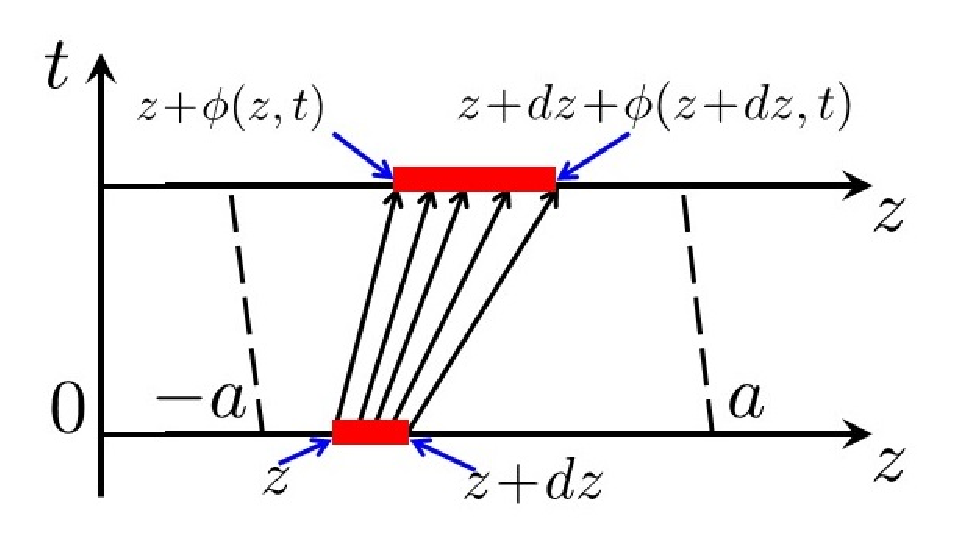
\includegraphics[width=0.5\columnwidth]{displacement_2}
\caption{(color online)
The definition of the displacement field $\phi(z,t)$ in Lagrangian formulation. 
At the time, shown as vertical axis, $t=0$ the fluid is contained in the interval $|z|<a$.
As time progresses the particles of a fluid move as indicated by narrow arrows pointing upward.
The particle located at $z$ at $t=0$ is shifted to the new position $z+\phi(z,t)$. 
A fluid volume shown as a narrow (red) horizontal rectangle occupies a segment $[z,z+dz]$ at time $t=0$.
At a later time $t>0$ this volume is displaced and occupies the segment $[z+\phi(z,t),z+dz+\phi(z+dz,t)]$.
The fluid volume expands (shrinks) if $\partial \phi(z,t)/ \partial z > (<) 0$.
The expansion (shrinkage) translates in the decrease (increase) in the density respectively.\cite{Iqbal2}}
\label{Fig-phi}
\end{centering}
\end{figure}


It should be noted that this segment is from $z$ to $z + d z$ in Lagrangian coordinates.
The force due to the pressure gradient is
\be\label{F_P}
F_P = P'(z + \phi(z,t)) - P'(z + d z + \phi(z + d z,t))
\ee
We assume that the pressure is the function of the density.
Then according to \eqref{hydro1} 
\be
P'(z+ \phi(z,t)) = P ( n'(z + \phi(z,t))) = P( \frac{ n(z) }{ 1 + \partial_z \phi(z,t)})
\ee
By the same token,
\be
P'(z+d z + \phi(z + dz,t)) = P ( n'(z+dz + \phi(z+dz,t))) = P( \frac{ n(z+dz) }{ 1 + \partial_z \phi(z+dz,t)})
\ee
Therefore the force is
\be
F_{P} = - \partial_z P(\frac{n(z)}{1 + \partial_z \phi(z,t)}) d z
\ee

\subsection{Force Due to the Confinement Potential}

The force due to the confinement potential, $U(z)$ exerted on the segment occupying the strip from $z$ to $z + dz$ in Lagrangian coordinates is 
\be
F_c = - \partial_z U(z + \phi(z,t)) n'(z + \phi(z,t)) d z = - \partial_z U(z + \phi(z,t)) n(z) d z
\ee

\subsection{Viscous Forces}

These forces conserve the total momentum, but roughly cause its diffusion.
Consider again the same parcel of a fluid.
The net force due to the viscosity in the leading in $\phi$ approximation reads
\be
\begin{split}
\label{vis_force}
- \eta(z+dz + \phi(z + dz)) \partial_z v[ z+dz + \phi(z + dz)] + 
\eta(z+ \phi(z )) \partial_z v[ z + \phi(z)] \\
\approx 
- 
\partial_z [\rho(z) \mu(z) \partial_z \partial_t \phi(z,t)]
\end{split}
\ee
Here we denote by $\eta(z)$ dynamic viscosity and $\mu(z) = \eta(z) / \rho(z)$ the kinematic viscosity.






\subsection{Newton's Law for Ideal fluid}
The acceleration of this same segment of fluid is
\be
a(z,t) = \partial^2_t \phi(z,t)
\ee

For a given parcel of a fluid  of a mass $n(z) m d z$, the Newton Law gives,
\be
m n(z) \partial_t^2 \phi(z,t) = - \partial_x P( \frac{ n(z) }{ 1 + \partial_z \phi(z,t)} ) - \partial_z U(z + \phi(z,t)) n(z)
\ee
This equation is exact. Linearizing in the displacement field $\phi$ we get,
\be
n(z,t) \approx n(z) - n(z) \partial_z \phi(z,t)
\ee
%\be
%P( \frac{ n(z) }{ 1 + \partial_z \phi(z,t)} ) \approx P ( n(z) - n(z) \partial_z \phi(z,t)) \approx P(n(z)) - \frac{\partial P(n(z))}{\partial n(z)} n(z) \partial_z \phi
%\ee
%\be
%\partial_z U(z + \phi(z,t)) n(z) \approx \partial_z U(z) n(z) + \partial^2_z U(z) n(z) \phi(z,t)
%\ee
The linearized equation of motion is given by:
\begin{align}
\label{hydro39}
&m n(z) \partial_t^2 \phi(z,t) = \notag \\
&-\partial_z P(n(z)) + \partial_z \left[  \frac{\partial P(n(z))}{\partial n(z)} n(z) \partial_z \phi(z,t)\right]
-\partial_z U(z) n(z) - \partial^2_z U(z) n(z) \phi(z,t)
\end{align}
At equilibrium we must get,
\be\label{hydro41}
0 = -\partial_z P(n(z)) -\partial_z U(z) n(z) = - \frac{ \partial P(n)}{\partial n } \frac{ \partial n(z) }{\partial z} - \partial_z U(z) n(z)
\ee

%We can write \eqref{hydro39} as
%\be\label{hydro47}
%m n(z) \partial_t^2 \phi(z,t) = 
%\partial_z \left[  \frac{\partial P(n(z))}{\partial n(z)} n(z) \partial_z \phi(z,t)\right]
% - \partial^2_z U(z) n(z) \phi(z,t)
%\ee
%Rewrite the second term as
%\be\label{hydro49}
%\partial_z \left[  \frac{\partial P(n(z))}{\partial n(z)} n(z) \partial_z \phi(z,t)\right]
%=
%n(z) \partial_z \left[  \frac{\partial P(n(z))}{\partial n(z)}  \partial_z \phi(z,t)\right]
%+ 
% \left[ \partial_z n(z) \right] \frac{\partial P(n(z))}{\partial n(z)} \partial_z \phi(z,t)
%\ee
%Using \eqref{hydro41}, \eqref{hydro49} becomes 
%\be\label{hydro51}
%\partial_z \left[  \frac{\partial P(n(z))}{\partial n(z)} n(z) \partial_z \phi(z,t)\right]
%=
%n(z) \partial_z \left[  \frac{\partial P(n(z))}{\partial n(z)}  \partial_z \phi(z,t)\right]
%-\partial_z U(z) n(z)  \partial_z \phi(z,t)
%\ee
%Substituting \eqref{hydro51} in \eqref{hydro39} allows to rewrite \eqref{hydro39} after canceling the equilibrium density $n(z)$ as
%\be\label{hydro53}
%m \partial_t^2 \phi(z,t) = 
%\partial_z \left[  \frac{\partial P(n(z))}{\partial n(z)}  \partial_z \phi(z,t)\right]
%-\partial_z U(z)  \partial_z \phi(z,t)
% - \partial^2_z U(z) \phi(z,t)
%\ee
After applying the equilibrium condition, equation \eqref{hydro39} can be rewritten as
\be\label{hydro55}
 \partial_t^2 \phi(z,t) = 
\partial_z \left[  \frac{\partial P(\rho(z))}{\partial \rho(z)}  \partial_z \phi(z,t)\right]
-\partial_z U_c(z)  \partial_z \phi(z,t)
 - \partial^2_z U_c(z) \phi(z,t)
\ee
The mass density, $\rho(z) = m n(z)$ and the partial derivative of the pressure in the right hand side of \eqref{hydro55} is understood as adiabatic as the fluid is assumed to be ideal.
We therefore define the local speed of sound as
\be
v_s^2 = \frac{\partial P(\rho(z))}{\partial \rho(z)} 
\ee
and look for the solutions in the form,
\be
\phi(z,t) = e^{- i \omega t } \phi(z)
\ee
so we get from \eqref{hydro55}
\be\label{hydro63}
 \omega^2 \phi(z) = 
- \partial_z \left[ v_s^2( n(z))  \partial_z \phi(z)\right]
+\partial_z U_c(z)  \partial_z \phi(z)
 + \partial^2_z U_c(z) \phi(z)
\ee

We consider a velocity Potential, $\chi(z)$ satisfying $\phi(z) = \chi'(z) = d\chi/ d z$.
With this potential \eqref{hydro63} takes the form,
\be\label{hydro65}
 \omega^2 \chi'(z) = 
- \partial_z \left[ v_s^2( n(z)) \chi''\right]
+\partial_z U_c(z)  \chi''
 + \partial^2_z U_c(z) \chi'
 =
 \partial_z \left[ - v_s^2( n(z)) \chi''  + \partial_z U_c(z)\chi' \right]
\ee
After removing one derivative by integration back over $z$ we get,
\be\label{hydro67}
 \omega^2 \chi + v_s^2( n(z)) \chi''-\partial_z U_c(z)  \chi'
 =0
\ee
\section{Exactly Solvable Cases}
Here we point out some solutions of linearized equation of an ideal fluid that are relevant for us.
\subsection{Kohn Mode in Hydrodynamics}
If we have a parabolic confinement potential $U_c = \omega_{\perp}^2 \frac{z^2 }{2}$, we get for the Euler equation,
\be\label{hydro69}
 \omega^2 \chi + v_s^2( n(z)) \chi''-\omega_{\perp}^2 z \chi'
 =0
\ee
The Kohn mode is then given by $\chi = \alpha z$ with $\omega = \omega_{\perp}$ regardless of the functional form of the sound velocity, $v_s^2$
%\subsection{Extended System, $\mathrm{U_c = const}$}
For an extended system with the confinement potential, $\mathrm{U_c = const}$, we just get the wave equation,
\be\label{hydro71}
 \omega^2 \chi + v_s^2 \chi'' =0
\ee
as it should be for linearized hydrodynamics of compressible and ideal fluid.
\subsection{Free Degenerate 2D Ideal Fermi Gas at $T=0$ in Parabolic Well}
This is the limit of primary interest to us.
Strictly speaking the hydrodynamics requires collisions and we assume that from the point of view of collisions our gas is not ideal.
But the Fermi liquid renormalizations are neglected here.
Spin is ignored too.

Let us fix the Fermi energy, $E_F$.
Then the maximal kinetic energy is reached at the center of the channel, and the gas occupies the strip of a width $2a$, where
\be\label{hydro77}
a =  \sqrt{ \frac{2 E_F}{ m \omega_{\perp}^2}}\, .
\ee
We therefore have for our gas from \eqref{hydro69} and \eqref{hydro75}
\be\label{hydro91}
 \omega^2 \chi + \frac{ \omega_{\perp}^2 }{2} (a^2 -z^2) \chi''-\omega_{\perp}^2 z \chi'
 =0
\ee
Now redefine the length scale $z \rightarrow z/a$,  multiply by $2/\omega_{\perp}^2$ and define
\be\label{hydro93}
\lambda_{\omega}^2 =2 \frac{\omega^2}{\omega_{\perp}^2 }
\ee
This makes \eqref{hydro91} to look as the Legendre equation,
\be\label{hydro91a}
 \lambda_{\omega}^2 \chi + (1 -z^2) \chi''-2 z \chi'
 =0
\ee
we therefore read off the solutions.
\be\label{hydro94}
\lambda_{\omega_n}^2 = 2 \frac{\omega_n^2}{\omega_{\perp}^2 } = n(n+1)
\ee
with $n=0,1,...$
so that the frequencies are
\be\label{hydro95}
\omega_n = \omega_{\perp} \sqrt{ \frac{ n(n+1)}{2}}
\ee
$n=0$ gives a ground state since as $\chi = const$, the velocity is identically zero.
$n=1$ is a Kohn mode as $P_1(z) = z$ is indeed linear.
We were able to get the whole hierarchy  of eigenoscilations of an electronic weakly interacting liquid.
They are Legendre polynomials,
\be
\chi_n(z/a) = \sqrt{\frac{ 2 n +1}{2}}P_n(z/a)
\ee
and the velocity fields are
\be
v_n(z/a) =   \partial_z P_n(z/a)\, .
\ee
\section{Depolarization Shift for the Kohn Mode in Ideal Fluid with Finite Non-Parabolicity}
We consider a weak anharmonicity,
\be\label{hydro96}
U_c(z) = \omega_{\perp}^2 \frac{z^2 }{2} + \frac{\epsilon}{4 m} z^4 + \delta U_c
\ee
where the constant $\delta U_c \propto \epsilon $ is added  in such a way that the spatial extent of the electronic liquid stays the same as for $\epsilon =0$.
In other words, 
\be
\delta U_c + \frac{\epsilon}{4 m} a^4 = 0
\ee
This is in fact not necessary, but convenient.
The convenience achieved this way is the absence of 
$\delta$-function contribution to the density, $\delta \rho \propto \delta(z \pm a)$.
We reconsider the Euler equation, \eqref{hydro67}.
It requires two modifications.
The first modification comes from the third term which becomes now according to \eqref{hydro96},
\be\label{hydro97}
-\partial_z U_c(z)  \chi' = \omega_{\perp}^2 z  + \frac{\epsilon}{ m} z^3\, .
\ee
The second modification is due to the change in the speed of sound which now reads
\begin{align}\label{hydro98}
v_s^2(z) & = \frac{1}{2} v_F^2(z) = \frac{1 }{ m } E_F(z) = 
\frac{1}{m} (E_F - \frac{ k z^2 }{2} - \frac{\epsilon}{4} z^4 - \delta U_c ) 
\notag \\
& =
\frac{k}{ 2 m} (a^2 - z^2- \frac{\epsilon}{2 m \omega_{\perp}^2} z^4+\frac{\epsilon}{2 m \omega_{\perp}^2} a^4) = \frac{ \omega_{\perp}^2 }{2} (a^2 -z^2) -
\frac{ \omega_{\perp}^2 }{2} \frac{\epsilon}{2 m \omega_{\perp}^2} (z^4 - a^4)
\end{align}
As a result the second term of \eqref{hydro67} takes the form,
\begin{align}
v_{s}^2 \chi'' = \frac{ \omega_{\perp}^2 }{2} (a^2 -z^2)\chi'' -
\frac{ \omega_{\perp}^2 }{2} \frac{\epsilon}{2 m \omega_{\perp}^2} (z^4-a^4) \chi''
\end{align}
Finally instead of the rescaled equation \eqref{hydro91} we obtain a modified equation,
\be\label{hydro101}
 \lambda_{\omega}^2 \chi + (1 -z^2) \chi''  -2 z \chi' 
 -
 \frac{\epsilon a^2 }{2 m \omega_{\perp}^2} (z^4 - 1) \chi''
 - \frac{2 a^2 \epsilon}{m \omega_{\perp}^2} z^3 \chi' 
 =0
\ee
We present it in the form,
\be\label{hydro101a}
 \lambda_{\omega}^2 \chi + (1 -z^2) \chi''  -2 z \chi' 
+V_{pert}^{\epsilon} [\chi] =0
 \ee
 where the perturbation reads
 \be\label{hydro101b}
 V_{pert}^{\epsilon} [\chi] = 
 -\frac{\epsilon a^2 }{2 m \omega_{\perp}^2}
 ( (z^4 - 1) \partial_z^2+  4 z^3 \partial_z )\chi =
  -\frac{\epsilon a^2 }{2 m \omega_{\perp}^2}
\partial_z[  ( (z^4-1) \partial_z )\chi]
\ee
It is absolutely crucial that $V_{pert}^{\epsilon}$ is Hermitian.
It follows from the simple observation that the anharmonicity alone causes the frequency shift but not a dissipation of the eigenmodes.
It also holds for any anharmonicity, 
% after the change, 
%$\partial_z[(z^4 -1)\partial_z \chi(z)] \rightarrow  \partial_z[(U_c^{anhar}(z) - U_c^{anhar}(a))\partial_z \chi(z)]$.
and in principle all the results on shift are generalizable to any anharmonic potential. 

It is crucial that the addition of $\delta U_c$ in \eqref{hydro96} modifies neither these conclusions  nor the final results.
Without this term thing would get messy because of the $\delta$-functions added to the density as described above.

To the leading order in $\epsilon$ we write,
\be
\lambda^2_{\omega_1} = 2 + \delta \lambda_1^2
\ee
where 
\be
\delta \lambda^2 = 2 \frac{\epsilon}{m \omega_{\perp}^2} 
\frac{ 2 *1 +1}{ 2 } a^2 \langle P_1(z)|\frac{1}{4} (z^4-1) \partial_z^2 + z^3 \partial_z| P_1(z)\rangle
\ee
here, dimensions were restored, and $a$ defined by \eqref{hydro77} is the size of the fermion cloud.
We now notice that
\be
\langle P_1(z)| \frac{1}{4} (z^4-1) \partial_z^2 + z^3 \partial_z| P_1(z)\rangle = \frac{2}{5}
\ee
so that
\be
\delta \lambda_1^2 = 2 \frac{\epsilon a^2}{m \omega_{\perp}^2} 
\frac{ 3}{ 2 }\frac{2}{5} = 
\frac{ 6 a^2}{5}\frac{\epsilon}{m \omega_{\perp}^2} 
\ee
Therefore
\be
2 \frac{\omega^2_1 }{ \omega_{\perp}^2} \approx 2 + \frac{ 6 a^2 }{5}\frac{\epsilon}{m \omega_{\perp}^2} 
\ee
and the correction to the Kohn mode frequency, $\delta \omega_1$ to the leading order in anharmonicity is
\be\label{hydro149}
\boxed{\frac{\delta \omega_1}{\omega_{\perp}} = \frac{ 3}{10}\frac{\epsilon a^2}{m \omega_{\perp}^2} }
\ee
We can also write it more explicitly using \eqref{hydro77} as 
\be
\boxed{\frac{\delta \omega_1}{\omega_{\perp}} = \frac{ 3}{5}\frac{ \epsilon E_F}{ (m \omega_{\perp}^2)^2} }
\ee

It can be explicitly verified that this result agrees with what one would get following the approach of \cite{Pantel2012}.


\section{Viscosity: Normal Modes Dissipation}
Here we analyze how the normal modes we found before get a finite relaxation time due to the processes of internal friction, i.e. the viscosity.
And start with the equation \eqref{hydro39} modified to include the viscous force, Eq.~\eqref{vis_force},
\begin{align}
\label{V14}
m n(z) &\partial_t^2 \phi(z,t) = \notag \\
 &\partial_z \left[  \frac{\partial P(n(z))}{\partial n(z)} n(z) \partial_z \phi(z,t)\right] - \partial^2_z U(z) n(z) \phi(z,t) - 
\partial_z [\rho(z) \mu(z) \partial_z \partial_t \phi(z,t)]
\end{align}
In terms of the velocity potential, we get instead of \eqref{hydro65}, %and assuming a constant $\eta$,
\be\label{V15}
 \omega^2 \chi'(z) = 
 \partial_z \left[ - v_s^2( n(z)) \chi''  + \partial_z U_c(z)\chi' \right]
 -
 i \omega  \frac{1}{  n(z)} \partial_z ( \mu(z) n(z) \partial_z^2 \chi(z))
\ee
 Integration over $z$ gives
 \be\label{V15}
 \omega^2 \chi(z) = 
 \left[ - v_s^2( n(z)) \chi''  + \partial_z U_c(z)\chi' \right]
 -
 i \omega \int_b^z \frac{d z }{  n(z)} \partial_z (\mu(z) n(z) \partial_z^2 \chi(z))
\ee
where the lower limit of the integral, $b$ is arbitrary.
It will be important to show that the final results are not dependent on $b$. 
We now make the same manipulations leading to Eqs.~\eqref{hydro101a} and \eqref{hydro101b} in Eq.~\eqref{V15}
\be\label{hydro101a}
 \lambda_{\omega}^2 \chi + (1 -z^2) \chi''  -2 z \chi' 
+V_{pert}^{\epsilon} [\chi] + V_{pert}^{\eta} [\chi] =0
 \ee
where the perturbation, $V^{\epsilon}_{pert}$ is defined by Eq.~\eqref{hydro101b}, and 
\be\label{V301}
V_{pert}^{\eta} [\chi] =  -
 i \omega \frac{2 \mu_0 }{ a^2 \omega_{\perp}^2} \int_b^z \frac{d z }{  n(z)} \partial_z (\bar{\mu}(z) n(z) \partial_z^2 \chi(z))
\ee
where $\mu_0 = \mu(z=0)$, and $\bar{\mu}(z) = \mu(z)/\mu_0$.
The exact $z$-dependence of $\mu(z)$ is not essential, and changes the numbers in finite results.
For the Fermi liquid $\eta \propto \rho v_F \ell$, $\ell \propto v_F E_F/T^2$,
\be\label{na}
\mu = \eta/\rho \propto  v_F^2 E_F/ T^2 = C_{\mu} n^2/(m^3 T^2) 
\ee
from \eqref{na} with $C_{\mu}>0$ a numerical constant.
It follows that 
\be\label{FL_mu}
\mu_0 = C_{\mu} \frac{ n^2(z=0)}{ m^3 T^2}\, ,\quad \bar{\mu}(z) = (1-z^2)^2
\ee
Using the definition, \eqref{hydro94} and introducing a constant 
\be
B =  \frac{\sqrt{2} \mu_0 }{ a^2 \omega_{\perp}} 
\ee
we put \eqref{V301} in the form 
\be\label{V301}
V_{pert}^{\eta} [\chi] =  -
 i \lambda_{\omega} B \int_b^z \frac{d z }{  n(z)} \partial_z (\bar{\mu}(z) n(z) \partial_z^2 \chi(z))
 =
 -
 i \lambda_{\omega} B \int_b^z \frac{d z }{ 1-z^2} \partial_z [(1-z^2)^3 \partial_z^2 \chi(z)]
\ee
\subsubsection{Perturbation Theory: Kohn Mode
% to Order $ \epsilon^0 \eta^n$ with Arbitrary $n=1,2,\ldots$
}
For the order of $ \epsilon^0 \eta^n$ with Arbitrary $n=1,2,\ldots$, we note that the Kohn mode is unaffected by viscosity at $\epsilon=0$, to any order in viscosity since,
\be\label{V303}
V_{pert}^{\eta} [\chi_1] =0
\ee
as expected from the Galilean invariance. Now we will investigate what happens at finite $\epsilon$.

%\subsubsection{Perturbation theory: Kohn mode to order $\epsilon^1 \eta^n$ with arbitrary $n=1,2,\ldots$}

We consider first $\epsilon^1 \eta^1$ order.
We know that the Kohn mode is shifted in frequency and at the same time acquires a finite admixture of the higher modes.
To the order $\epsilon \eta$ we have the following correction to $\lambda_{\omega_1}$,
\begin{align}
\label{V307}
\delta \lambda^2_1 = - i \lambda_{\omega} B  \sum_{n=1}^{\infty}& 
\frac{\sqrt{ 3/2 }\sqrt{(2 n +1)/2}}{2 - n(n+1)} \notag \\
&\left[
\langle P_1| V_{pert}^{\eta} | P_n\rangle \langle P_n| V_{pert}^{\epsilon} | P_1 \rangle
+
\langle P_1| V_{pert}^{\epsilon} | P_n\rangle \langle P_n| V_{pert}^{\eta} | P_1 \rangle \right]
\end{align}
Among the two terms in \eqref{V307} the second vanishes according to \eqref{V303}.
The first term vanishes as well,
\begin{align}
\langle P_1| V_{pert}^{\eta} | P_n\rangle & \propto
\int_{-1}^{1} d x P_1(x) \int_{b}^x d z \frac{1}{n(z)} \partial_z(n^3(z) \partial^2_z P_n(z)
\notag \\
&=\frac{1}{2} \int_{-1}^{1} d x \partial_x n(x) \int_{b}^x d z \frac{1}{n(z)} \partial_z [n(z)^3 \partial^2_z P_n(z)]
\notag \\
&=
-\frac{1}{2} \int_{-1}^{1} d x n(x)  \frac{1}{n(x)} \partial_x [n^3(x) \partial^2_z P_n(x)]
\notag \\
&=
-\frac{1}{2} \int_{-1}^{1} d x  \partial_x [n^3(x) \partial^2_x P_n(x)]
=0
\end{align}
regardless of $b$ and $n$.
It may be noted that the cancellation is not specific to the model of viscosity, it will hold as long as $\eta=0$ in the limit of $\rho =0$ which is quite natural: in the absence of particles there no carriers of momentum.
It follows that the correction to the frequency vanishes to any order to $\epsilon \eta^n$ with $n=1,2,\ldots$.



This is an important observation, as in the case we had a finite result, the new energies would be found from $\omega_1^2 = 2 + i \eta \epsilon \omega_1 $ which gives the imaginary part to $\omega_1$ that has the sign determined by the sign of $\epsilon$ which is an impossible conclusion.

%\subsubsection{Perturbation theory: Kohn mode to order $\epsilon^2 \eta^1$.} 
The leading non-vanishing correction comes from the order $\epsilon^2 \eta^1$ term.
According to the perturbation theory the third order correction is given by 
\begin{align}
\delta E^{(3)}_0 = \sum_{k \neq 0}\sum_{m \neq 0} \frac{ \langle 0 | V |m \rangle \langle m | V | k \rangle \langle k  | V | 0\rangle}
{(E_m - E_0)(E_k - E_0)}
-
\langle 0 | V | 0 \rangle  \sum_{m \neq 0} \frac{ \langle 0| V | m\rangle  \langle m| V | 0 \rangle}{ (E_m - E_0)^2 } 
\end{align}
Identifying $|0\rangle = | P_1 \rangle$ as a Kohn mode, and $V = V_{pert}^{\eta} + V_{pert}^{\epsilon}$ and noting that in general
\be
\langle P_1 | V_{pert}^{\eta} | P_n \rangle = \langle P_n | V_{pert}^{\eta} | P_1 \rangle = \langle P_1 | V_{pert}^{\epsilon} | P_1 \rangle = 0, \mathrm{for\, all}\, n
\ee
and for quartic anharmonicity in particular the only non-zero off-diagonal matrix elements are, using \eqref{hydro101b} is $\langle P_1 | V_{pert}^{\epsilon} | P_3 \rangle = \langle P_3 | V_{pert}^{\epsilon} | P_1 \rangle$ with the rest of the matrix elements $\langle P_n | V_{pert}^{\epsilon} | P_1 \rangle =0 $ for $n\neq 1,3$.
We thus have, including the normalization factors,
\be
\delta^{(3)} \lambda_{\omega_1}^2 = \frac{ \langle   P_1| V_{pert}^{\epsilon} | P_3 \rangle \langle  P_3 | V_{pert}^{\eta} | P_3 \rangle \langle P_3 |V_{pert}^{\epsilon} | P_1 \rangle }{ (\lambda_1^2 - \lambda_3^2)^2} \frac{ 2 *1 + 1}{2} \left(\frac{2*3 + 1}{2}\right)^2
\ee
where $\lambda_1^2 = 1(1+1)=2$ and $\lambda_3^2 = 3(3+1)=12$ 
and  $(\lambda_1^2 - \lambda_3^2)^2 = 10^2$.
Using the explicit expressions  \eqref{V301}, \eqref{hydro101b} , and the numbers,
\begin{align}
\label{PT101}
 \int_{-1}^1 d z P_3(z) \int_b^z \frac{d x }{ 1-x^2} \partial_x [(1-x^2)^3 \partial_x^2 P_3(x)] &= - \frac{40}{21}\notag \\
 \int_{-1}^1 d z P_1(z) \partial_z [(z^4 - 1)\partial_z P_3(z)] &= \frac{8}{5}
\end{align}
along with the definition \eqref{hydro93}
\begin{align}
\delta^{(3)} \lambda_{\omega_1}^2 = 
\delta^{(3)} 2 \frac{\omega^2}{ \omega_{\perp}^2} =
- i \lambda_{\omega} \frac{\sqrt{2} \mu_0 }{ a^2 \omega_{\perp}} \left(\frac{\epsilon a^2 }{2 m \omega_{\perp}^2}\right)^2 ( - \frac{40}{21}) \left(\frac{8}{5}\right)^2 \frac{3}{2} (\frac{7}{2})^2 10^{-2}
\end{align}
For now omitting the numerical prefectures we get
\begin{align}
\frac{\delta \omega}{\omega_{\perp}} = i \frac{\mu_0 }{ a^2 \omega_{\perp}} 
\left(\frac{\epsilon a^2 }{ m \omega_{\perp}^2}\right)^2 
= i \frac{ \mu_0 \epsilon^2 a^2 }{m^2 \omega_{\perp}^5}
\end{align}
The relaxation rate for the mode,
is 
\begin{align}
\boxed{\frac{1}{\tau_{Kohn}} \propto \frac{ \mu_0 \epsilon^2 a^2 }{m^2 \omega_{\perp}^4}}
%= \frac{  \epsilon^2 a^4 }{m^2 \omega_{\perp}^4} \frac{\mu_0}{a^2}
\end{align}
To interpret this result we use the expression \eqref{hydro149} to write it in the form,
\begin{align}\label{res_life}
\boxed{\frac{1}{\tau_{Kohn}} \propto \left(\frac{ \delta \omega_1}{\omega_{\perp}} \right)^2 \frac{\mu_0}{a^2}}
\end{align}
which has a straightforward interpretation.
The higher modes not protected by the Kohn theorem decay with the rate,
$ \mu_0 / a^2 $ as $\mu_0$ has dimensions of the diffusion coefficient.
This is the typical rate of momentum relaxation. 
The ratio  $\left(\frac{ \delta \omega_1}{\omega_{\perp}} \right)^2$ is the probability of finding the system in higher modes.

\section{Solution of Navier-Stokes equations}
A hydrodynamic description is based on the existence of slow variables associated with locally conserved quantities such as number of particles, momentum and energy. The motion of the liquid is described by the Navier-Stokes equations which in Eulerian continuous field coordinates can be put in the form~\cite{LL} 
\begin{equation}\label{E-eq}
\partial_t(\rho v_j)=-\partial_i\Pi_{ij}-\rho\partial_jU,
\end{equation}
that guaranties the momentum conservation, which holds in ideal and nonideal liquids alike in the absence of confining potential $U$. The stress tensor of a two-dimensional fluid giving rise to the Navier-Stokes equation is~\cite{LL} 
\begin{equation}\label{Pi}
\Pi_{ij}=\delta_{ij}P+\rho v_iv_j-\zeta\delta_{ij}\partial_kv_k
-\eta(\partial_iv_j+\partial_jv_i-\delta_{ij}\partial_kv_k).
\end{equation}
Here $\eta,\zeta$ are the first (shear) and second (bulk) viscosities, and $P$ is pressure. In the following we focus on a one-dimensional flow in $z$-direction of a two-dimensional liquid occupying the strip $|z|<a$, so that velocity vector field can be taken in the form $\bm{v}=v(z,t)\bm{e}_z$ and Eq.~(\ref{E-eq}) simplifies to 
\begin{equation}\label{NS-eq}
\rho(\partial_t v+v\partial_zv)=-\partial_z P-\rho \partial_z U+\partial_z(\eta\partial_zv).
\end{equation}  
When writing this equation we made use of the continuity equation $\partial_t\rho+\partial_z(\rho v)=0$ and employed standard assumption $\eta\gg\zeta$. For the purpose of our study it will be convenient to use a particle description of Navier-Stokes equation.
In this approach the coordinate $z$ labels an equilibrium position of a fluid particle, and its location at later time $t$ is the $z+ \phi(z,t)$ such that $\phi$ is the displacement field.
By definition, the density is $\rho(z+\phi(z,t),t) = \rho_0(z)/ ( 1 + \partial_z \phi(z,t))$, the velocity $v(z+\phi(z,t)) = \partial_t \phi(z,t)$.
The linearization of Eq.~\eqref{NS-eq} is equivalent to the linearization in $\phi$.
To the leading order, 
\begin{align}\label{leading}
\rho = \rho_0 + \delta \rho\, ,\,\, \delta \rho  = 
- (\rho_0 \phi)'  \, , \quad  v = \dot{\phi} \, ,
\end{align}
where $\rho_0$ is a stationary equilibrium density distribution, the notations $f' = \partial f/ \partial z$ and $\dot{f} = \partial f / \partial t$ are introduced and the pair of arguments $(z,t)$ common to all the functions is omitted.  
The parametrization \eqref{leading} of $\delta \rho$ and $v$ by a single displacement field automatically satisfies the linearized continuity equation, $\delta \dot{\rho} + (\rho_0 \dot{\phi})' = 0$.
The concept of the displacement field is further illustrated in Fig.~\ref{Fig-phi}. For the solutions of the form $\phi(z,t) = e^{i \omega t} \chi'(z)$ the equation \eqref{NS-eq} in the parameterization, \eqref{leading} reads, (see Appendix \ref{App2}):
\begin{equation}\label{normal-modes-eq}
\omega^2\chi=-v^2_s\chi''+U'\chi' -i\omega\int^{z}_{z_0}\frac{dz}{\rho_0}(\nu \rho_0 \chi'')',
\end{equation}
where $\nu(z)=\eta(z)/\rho_0(z)$ is the kinematic viscosity, and
\begin{align}\label{v_s}
v_s=\sqrt{\partial P/\partial\rho_0}
\end{align}
has a meaning of a local speed of sound that depends on $z$ only through the equilibrium density $\rho_0$. We show that the results are independent on arbitrary $z_0$.

The spectrum of collective excitations and their decay rates as given by Eq.~\eqref{normal-modes-eq} depend on the details of the confining potential and dependence of the viscosity on density. 
Here for definiteness we consider the confining potential per unit mass with a weak quartic anharmonicity,
\begin{equation}\label{U}
U=\frac{\omega^2_\perp z^2}{2}+\frac{\epsilon z^4}{4m}+\delta U,
\end{equation}
where $m$ is the mass of an individual particles, and the constant $\delta U\propto\epsilon$ is added in such a way that the spatial extent of the liquid stays the same as for $\epsilon=0$. In other words $\delta U+\epsilon a^4/4m=0$. This choice is not obligatory, yet convenient in the further calculations. 
The anharmonic part $\propto\epsilon$ of $U$ not only modifies the second term in the right-hand-side of Eq.~(\ref{normal-modes-eq}) but also the first one. Indeed, in the parabolic confinement the sound velocity is $v^2_s(z)=2\pi \rho(z)/m^3=\omega^2_\perp(a^2-z^2)/2$, which acquires now a correction $\delta v^2_s(z)=-\epsilon(z^4-a^4)/4m$.  
With these observations in mind we multiply Eq.~(\ref{normal-modes-eq}) by $2/\omega^2_\perp$, rescale coordinates $z\to z/a$ and introduce $\lambda^2_\omega=2\omega^2/\omega^2_\perp$ to find 
\begin{equation}\label{eigenmodes}
\lambda^2_\omega\chi+(1-z^2)\chi''-2z\chi'+V_\epsilon+V_\nu=0.
\end{equation}
The perturbation term due to anharmonicity can be cast in the form 
\begin{equation}\label{V1}
V_\epsilon=-\frac{\epsilon a^2}{2m\omega^2_\perp}[ (z^4-1)\chi ']'.
\end{equation}
This formula can be generalized to any confining potential after the change $[(z^4-1)\chi']'\to [(U(z)-U(a))\chi']'$. Consequently, our results for the depolarization shift are straightforward to modify for arbitrary confinements. 
We emphasize that $V_\epsilon$ is Hermitian. 
This property guaranties that the anharmonicity alone causes only the frequency shift but no dissipation. We argue below that only the combination of the anharmonicity and viscosity leads to the dissipation of the Kohn mode. The exact $z$-dependence of the viscosity $\nu(z)$ is specific to the model. This however only influences the numerical prefactors in the final results and we take the expression for the viscosity from the theory of Fermi liquids, $\eta\propto v_F\rho\ell$, where mean fee path is $\ell\propto v_FE_F/T^2$ with $v_F$ and $E_F$ being Fermi velocity and energy, respectively. 
For this case $\nu(z)=C\rho^2(z)/m^5T^2$ where $C$ is the numerical factor of the order of unity~\cite{Abrikosov}. In the above specified dimensionless notations this results in 
\begin{equation}\label{V2}
V_\nu=-i\lambda_\omega B\int^{z}_{z_0}\frac{dz}{1-z^2}[(1-z^2)^3  \chi'']',
\end{equation}
where we have introduced $B=\sqrt{2}\nu_0/a^2\omega_\perp$ with $\nu_0=\nu(z=0)$. We proceed with the analysis of Eq.~(\ref{eigenmodes}). 

\section{Results}
As the first step let us discuss the eigenmodes of an ideal fluid confined to a harmonic trap. For that purpose we neglect anharmonicity and interaction effects implicit in the viscosity term of Eq.~(\ref{eigenmodes}), i.e. we set $V_{\epsilon} =V_{\eta}=0$. 
What remains is familiar Legendre equation and we therefore immediately read off its solutions $\lambda^2_{\omega_n}=2\omega^2_n/\omega_\perp=n(n+1)$ with $n=0,1,2,\ldots$ so that the eigenfrequencies are 
\begin{equation}\label{omega-n}
 \omega_n=\omega_\perp\sqrt{\frac{n(n+1)}{2}}. 
\end{equation}
The $n=0$ gives an equilibrium since $\chi_{n=0}=const$ this velocity is identically zero. The $n=1$ is a Kohn mode $\omega_1=\omega_\perp$. We thus found the whole hierarchy of eigenoscillations, they are Legendre polynomials 
\begin{equation}\label{chi}
\chi_n(z)=\sqrt{\frac{2n+1}{2}}P_n(z)
\end{equation} 
and the related velocity fields are $v_n(z)=\partial_zP_n$. 
Remarkably, the same spectrum of collective modes as \eqref{omega-n} was obtained recently for the longitudinal oscillations of the one-dimensional Coulomb chains \cite{Morigi_PRE}.
In this systems the collective behavior sets in due to the long range Coulomb forces rather than collisions.

Next we discuss the significance of perturbation terms on the spectrum of collective modes. Let us first consider anharmonicity alone, i.e. we set $V_{\eta}=0$ and $V_{\epsilon}\neq 0$ in Eq.~\eqref{eigenmodes}. As $V_{\epsilon}$ is Hermitian the spectrum remains real.
As a result all the eigenmodes remain undamped as expected in the absence of collisions.
To find the depolarization shift of the Kohn mode, $\delta^{(1)} \omega_1$ to the leading order in $\epsilon$ we write $\lambda^2_{\omega_1}=2+\delta^{(1)} \lambda^2_{\omega_1}$, where the correction term is found from the first order perturbation theory 
\begin{equation}
\delta^{(1)} \lambda^2_{\omega_1}=\frac{3\epsilon a^2}{4m\omega^2_\perp}\langle P_1(z)|(z^4-1)\partial^2_z+4z^3\partial_z|P_1(z)\rangle.
\end{equation}
The matrix element gives a factor of $8/5$ which eventually translates into the correction to the Kohn mode frequency 
\begin{equation}\label{dep_shift}
\delta^{(1)}\omega_1=\frac{3\epsilon a^2}{10m\omega_\perp}.
\end{equation}
We have checked that the result \eqref{dep_shift} agrees with the result obtained by the method of moments suggested in Ref.~\cite{Pantel2012}. We note however that the result for the depolarization shift in the collisioneless regime differ from Eq.~\eqref{dep_shift} by a nonuniversal numerical prefactor. 
For instance, for the contact interaction we obtain by direct perturbation theory in Fermions $\delta^{(1)}\omega_1=3\epsilon a^2/5m\omega_\perp$, \cite{Iqbal2}. Corrections to all other eigenfrequencies can be computed in the same fashion, which will have the same form as above but with the different numerical coefficients. 

Before considering the generic case, it is instructive to verify the Kohn's theorem within our hydrodynamic approach. It amounts to the statement that $\chi_1(z) \propto z$ remains the solution of Eq.~(\ref{eigenmodes}) with the frequency $\omega_1 = \omega_{\perp}$ even for $V_{\eta} \neq 0$ provided only $V_{\epsilon}=0$. This in turn will be proven once we show that for any non-negative $n$, $\langle P_1  | V_{\eta} | P_n \rangle = \langle P_n  | V_{\eta} | P_1 \rangle =0$. Clearly $V_{\eta} | P_1 \rangle =0$ as $[P_1(z)]''=0$. On the other hand from Eq.~(\ref{normal-modes-eq}) it follows that 
\begin{align}
\!\!\!\langle P_1|V_\nu| P_n\rangle \!\!\propto\!\!\int^{1}_{-1}\!\!\!\!d\bar{z} P_1(\bar{z})\!\!\! \int^{\bar{z}}_{z_0}\!\!\frac{dz}{\rho_0(z)}\{\nu(z) \rho_0(z) [P_n(z)]'\}'.
\end{align}
Realizing that $P_1(\bar{z})=-\partial_z \rho_0(\bar{z})/2$ and integrating by parts one concludes that $\langle P_1|V_\nu| P_n\rangle=0$ for all $n$ thus proving the Kohn theorem in the present context.

It follows that the Kohn mode may acquire a finite life-time only when the anharmonicity is included.
Yet the perturbation $V_{\epsilon}$ is Hermitian and by itself is insufficient.
We therefore consider both perturbations, and look for the corrections that are first order in each of the two. In the second order perturbation theory such a correction is of the form     
\begin{eqnarray}
&&\hskip-.25cm\delta^{(2)}\lambda^2_{\omega_1}=-i\lambda_\omega B\sum^{\infty}_{n=1}\frac{\sqrt{3/2}\sqrt{(2n+1)/2}}{2-n(n+1)}\nonumber\\
&&\hskip-.25\times[\langle P_1|V_\nu| P_n\rangle\langle P_n|V_\epsilon| P_1\rangle+
\langle P_1|V_\epsilon| P_n\rangle\langle P_n|V_\nu| P_1\rangle].
\end{eqnarray}
As we saw above both terms in this equation are zero as the Kohn mode does not couple to any other mode by a viscosity term $V_{\eta}$, and $\delta^{(2)}\lambda^2_{\omega_1}=0$.

Inevitably we have to consider the third order corrections to $\lambda_{\omega_1}$. 
The third order correction to the energy $E_l$ of a state $|l\rangle$ is 
\begin{eqnarray}
\delta^{(3)} E_l=\sum_{k,m\neq l}\frac{\langle l|V|m\rangle\langle m|V|k\rangle\langle k|V|l\rangle}{(E_m-E_l)(E_k-E_l)}\nonumber\\
-\langle l|V|l \rangle\sum_{m\neq l}\frac{\langle l|V|m\rangle\langle m|V|l\rangle}{(E_m-E_l)^2}. 
\end{eqnarray}
To apply this expression to our problem we identify $|l\rangle=P_1$ as a Kohn mode and $V=V_\epsilon+V_\nu$. We observe that for the perturbation terms given by Eqs.~(\ref{V1}) and (\ref{V2}) the following properties of matrix elements hold $\langle P_1|V_\nu|P_n\rangle=\langle P_n|V_\nu|P_1\rangle=\langle P_1|V_\epsilon|P_1\rangle=0$ for all $n$. Furthermore, for the quartic anharmonicity under consideration the only nonzero off-diagonal matrix elements are $\langle P_1|V_\epsilon|P_3\rangle=\langle P_3|V_\epsilon|P_1\rangle$ with the rest of matrix elements $\langle P_n|V_\epsilon|P_1\rangle=0$ for $n\neq1,3$. We thus have, accounting for all the normalization factors of eigenoscillation modes (\ref{chi}) 
\begin{equation}
\delta^{(3)}\lambda^2_1=\frac{147}{8(\lambda^2_1-\lambda^2_3)^2}\langle P_1|V_\epsilon|P_3\rangle
\langle P_3|V_\nu|P_3\rangle
\langle P_3|V_\epsilon|P_1\rangle.
\end{equation}
Using the explicit expressions (\ref{V1}) and (\ref{V2}) we find for the matrix elements 
\begin{eqnarray}
&&\hskip-.25cm\int^{1}_{-1}d\bar{z}P_3(\bar{z})\int^{\bar{z}}_{z_0}\frac{dz}{1-z^2}\partial_z[(1-z^2)^3\partial^2_zP_3]=-\frac{40}{21},\\
&&\hskip-.25cm\int^{1}_{-1}dz P_1(z)\partial_z[(z^4-1)\partial_zP_3(z)]=\frac{8}{5},
\end{eqnarray}
and eventually
\begin{equation}
\delta^{(3)}\lambda^2_1=i\lambda_\omega\frac{28\sqrt{2}}{125}\frac{\nu_0}{a^2\omega_\perp}
\left(\frac{\epsilon a^2}{m\omega^2_\perp}\right)^2.
\end{equation}
This result enables us to find imaginary part of the Kohn mode $\omega_1=\omega_\perp+\delta\omega_1+i\tau^{-1}_1$, which corresponds to its attenuation with the rate 
\begin{equation}\label{tau-K}
\tau^{-1}_1\simeq\frac{\nu_0\epsilon^2a^2}{m^2\omega^4_\perp}\simeq\left(\frac{\delta\omega_1}{\omega_\perp}\right)^2\frac{\nu_0}{a^2},
\end{equation}
where we omitted numerical factors of order unity for brevity. This expression constitutes the main result of our work and has straightforward interpretation. The higher excitations modes not protected by the Kohn theorem decay with the rate $\sim\nu_0/a^2$. As $\nu_0$ has dimensions of the diffusion coefficient, this is the typical rate of the momentum relaxation. The ratio $(\delta\omega_1/\omega_\perp)^2$ is the probability of finding the system in higher modes.    

 

